% Appendix to sec:tech-segment-glmm (content/technical/01_mixed_model.tex, renamed 2026-11-15 from 01_prediction_model.tex): cloglog against logit.
% Written 2026-11-14 (user: "add all of this to the appendix so the technical background just focuses on
%   the cloglog"), from reports/cloglog_vs_logit_simple. Rebuilt 2026-11-14 with the technical section
%   (user: "use the best of score2_loglog_explainer.pdf and cloglog_vs_logit.md"): merged in the draft
%   content/appendix/cloglog_rate.tex (deleted), i.e. the rate reading with a worked example, the
%   odds-ratio numbers and the sentence on the risk rising toward 1. General method only, present tense;
%   why this thesis uses cloglog is Methodology (05_statistical_model.tex), the caveats (PH untestable,
%   conditional hazard ratios) are Discussion.
% Sources: dobson2002glm (PDF read 2026-11-14): Section 10.2 Eq. 10.4 S = exp(-H); 10.2.2 Eqs. 10.7-10.9
%   proportional hazards, hazard ratio, log cumulative hazards differ by a constant; 10.2.3 Eq. 10.13
%   log H = log[-log S] (complementary log-log scale); 7.3 the cloglog link; 8.3 logistic coefficients as
%   log odds ratios. prentice1978grouped p. 66 for window-length independence.
% Own computation (Python, 2026-11-14), not from a source: 0.99^10 = 0.904 and -log = 0.1005;
%   Lambda for risks 0.05, 0.40, 0.90 = 0.051, 0.51, 2.30; with a constant reference hazard and hazard
%   ratio 1.5 the odds ratio is 1.51 at a 2% reference risk and 1.73 at 40%.
% CHECK: the asymmetry sentence (cloglog approaches 0 as the logit does, 1 much faster) is algebra of
%   the inverse links; confirm Dobson Section 7.3 shows it before citing it there.
% CHECK: "proportional odds" over time (the logit model holding for every window length) is reasoning,
%   uncited; Dobson's proportional odds model (8.4.2) is for ordered response categories, not time.
% CHECK: "odds do not add", "the risk rises toward 1" and "neither assumption can be tested with one
%   observation per unit" are reasoning, uncited.
% Figure: content/appendix/figures/link_ratios.py, made-up numbers (reference risk 40% by year 10, ratio
%   1.5); 40% rather than the cohort's 42%, which belongs to Results.
% 2026-11-15 (user: move the technical math of sec:tech-segment-glmm here): new section app:link-derivation (rate
%   example, 1 - p = exp(-Lambda), PH step eq:app-link-ph, link form eq:app-link-cloglog); the logit comparison is now
%   section app:link-logit. CHECK: Dobson 10.2.3 Eq. 10.13 for "log cumulative hazards differ by beta" (was cited 10.2.2).
% 2026-11-16 (user: "make an explanation of this in the appendix"): ADDED to app:link-derivation, after the
%   rare/common paragraph, a paragraph on exp(-Lambda) as a probability over all event times, one observation at
%   the end of the window, and Lambda (area) determined but not the shape of h_i(t). Uncited reasoning from
%   eq:tech-cumhaz (Dobson 10.2, Eq. 10.4 is cited in the paragraph above). Uses h_i(t) from eq:tech-cumhaz.
%   Overlaps with the last sentence of app:link-logit (time course of the ratios not observed): that sentence is
%   about the ratios, this one about the hazard; keep both or merge if the appendix is shortened.
%   Not added (offered to the user): the event must be irreversible, so no event at the end means none in the window.
\chapter{Choice of Link Function}
\label{app:link}

\section{Derivation of the Complementary Log-Log Link}
\label{app:link-derivation}

The complementary log-log (cloglog) link of Section~\ref{sec:tech-segment-glmm} describes the event through its rate.
If a unit has a probability of 0.99 of staying event-free through each year of a 10-year window, its probability of staying event-free through the whole window is $0.99^{10} = 0.904$.
Minus the logarithm of this product is the sum $10 \times (-\log 0.99) = 0.1005$, the hazard of each year added up over the window.
In general, the probability of no event by the end of the window is $1 - p_i = \exp(-\Lambda_i)$, so $\Lambda_i = -\log(1 - p_i)$ is the cumulative hazard \cite[Section~10.2, Eq.~10.4]{dobson2002glm}.
For a rare event the cumulative hazard is close to the probability, as a risk of 0.05 gives $\Lambda = 0.051$, while for a common event it grows faster, as a risk of 0.40 gives 0.51 and a risk of 0.90 gives 2.30.

The probability $\exp(-\Lambda_i)$ is derived from the hazard $h_i(t)$ of Eq.~\eqref{eq:tech-cumhaz}, which at each time applies to the units that are still event-free.
It therefore covers every time at which the event can occur within the window, and a unit needs to be observed only once, at the end of the window, to show whether it remained event-free.
Such data determine the cumulative hazard $\Lambda_i$, which is the area under $h_i(t)$, but not the shape of $h_i(t)$ over the window.
A hazard concentrated early in the window and a hazard concentrated late give the same risk when their areas are equal, so the data cannot distinguish them.

Let $\Lambda_0$ be the cumulative hazard over the window of a reference unit with every covariate at zero.
Under proportional hazards, the covariates of unit $i$ multiply its hazard at every time by the same factor, so they multiply its cumulative hazard by that factor too \cite[Section~10.2.2, Eqs.~10.7--10.9]{dobson2002glm},
\begin{equation}
  \Lambda_i = \Lambda_0 \exp\Bigl(\sum_k \beta_k x_{ik}\Bigr) = \exp(\eta_i),
  \qquad
  \beta_0 = \log \Lambda_0 .
  \label{eq:app-link-ph}
\end{equation}
Inserting Eq.~\eqref{eq:app-link-ph} into $1 - p_i = \exp(-\Lambda_i)$ gives the risk of Eq.~\eqref{eq:tech-cloglog}, and solving for $\eta_i$ gives the link itself \cite[Section~7.3]{dobson2002glm}, \cite[pp.~58--59, Eqs.~2--5]{prentice1978grouped},
\begin{equation}
  g(p_i) = \log\{-\log(1 - p_i)\} = \eta_i ,
  \label{eq:app-link-cloglog}
\end{equation}
the logarithm of minus the logarithm of the complement $1 - p_i$, which gives the link its name.
The log cumulative hazards of two units that differ only in $x_{ik}$ therefore differ by $\beta_k$, so $\exp(\beta_k)$ is a hazard ratio that stays the same over the whole window \cite[Section~10.2.3, Eq.~10.13]{dobson2002glm}.

\section{Comparison with the Logit Link}
\label{app:link-logit}

The logit link, the most common link for a binary outcome, also maps a linear predictor to a probability between 0 and 1.
The logit link is symmetric around a probability of 0.5, while the cloglog link is not: as the linear predictor decreases, the probability approaches 0 at the same pace as under the logit link, but as it increases, the probability approaches 1 much faster \cite[Section~7.3]{dobson2002glm}.
The two links differ in what they assume about how a covariate acts over the observation window.

Under the logit link, $\log\{p/(1-p)\} = \eta$, and $\exp(\beta_k)$ is the odds ratio for a one-unit increase in $x_k$ \cite[Section~8.3]{dobson2002glm}.
If this model holds for every length of window, the covariate multiplies the odds of having had the event by the same factor at every time, referred to as proportional odds.
Only one of the two ratios can be constant over time (Figure~\ref{fig:app-link}).
When the hazard ratio is held constant, the unit with the covariate keeps adding event probability at a fixed multiple of the reference rate, and as it pulls ahead its odds grow faster than its probability, so the odds ratio rises with time.
When the odds ratio is held constant, the hazard ratio instead falls toward 1, as a unit that already has a high event probability needs only a small further increase to keep its odds a fixed multiple of the reference.

\begin{figure}[htbp]
  \centering
  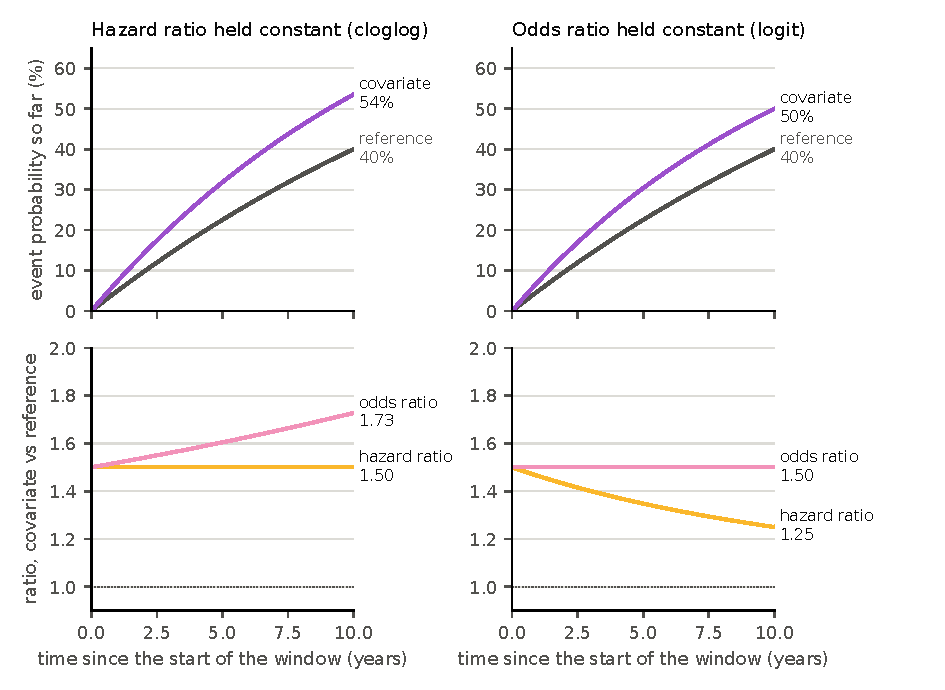
\includegraphics[width=\textwidth]{content/appendix/figures/link_ratios.pdf}
  \caption{Event probability over a 10-year window for a reference unit and a unit with a covariate (top), and the hazard ratio and odds ratio between them (bottom), when the hazard ratio is held at 1.5 (left, cloglog) or the odds ratio is held at 1.5 (right, logit). Made-up numbers: the reference unit has a constant hazard and a 40\% event probability by the end of the window.}
  \label{fig:app-link}
\end{figure}

The odds and the cumulative hazard are both close to the probability while events are rare, so the two ratios nearly coincide for rare events and part as events become common.
With a constant reference hazard and a hazard ratio of 1.5, the corresponding odds ratio is 1.51 when the reference unit has a 2\% event probability by the end of the window, but 1.73 when it has 40\%.
An odds ratio therefore changes with the baseline risk and with the length of the window, while the hazard ratio under proportional hazards does not \cite[p.~66]{prentice1978grouped}.

Rates can also be added, which odds cannot.
Given the cluster effect, the hazards of the units of a cluster add to one cluster hazard, so the cluster risk keeps the cloglog form (Eq.~\eqref{eq:tech-agg-conditional}).
A product of logistic terms is not logistic, so under the logit link the cluster risk has no such form and can only be computed unit by unit.

As long as the hazard is above zero, the cumulative hazard keeps growing with the length of the window, so the modelled risk rises toward 1 as the window is extended.
The model therefore describes risk over the window it is fitted to and says nothing about much longer windows.
With one observation per unit at the end of the window, the time course of the ratios is not observed, so neither proportional hazards nor proportional odds can be tested.
